%%% LaTeX Template: Newsletter
%%%
%%% Source: http://www.howtotex.com/
%%% Feel free to distribute this template, but please keep the referal to HowToTeX.com.
%%% Date: September 2011


%%% ---------------
%%% PREAMBLE
%%% ---------------
\documentclass[10pt,a4paper]{article}

% Define geometry (without using the geometry package)
\setlength\topmargin{-48pt}
\setlength\headheight{0pt}
\setlength\headsep{25pt}
\setlength\marginparwidth{-20pt}
\setlength\textwidth{7.0in}
\setlength\textheight{9.5in}
\setlength\oddsidemargin{-30pt}
\setlength\evensidemargin{-30pt}

\frenchspacing						% better looking spacing

% Call packages we'll need
\usepackage[english]{babel}			% english
\usepackage{graphicx}				% images
\usepackage{amssymb,amsmath}		% math
\usepackage{multicol}				% three-column layout
\usepackage{url}					% clickable links
\usepackage{marvosym}				% symbols
\usepackage{wrapfig}				% wrapping text around figures
\usepackage[T1]{fontenc}			% font encoding
\usepackage{charter} 				% Charter font for main content
\usepackage{blindtext}				% dummy text
\usepackage{datetime}				% custom date
	\newdateformat{mydate}{\monthname[\THEMONTH] \THEYEAR}
\usepackage[pdfpagemode=FullScreen,
			colorlinks=false]{hyperref}	% links and pdf behaviour

% Customize (header and) footer
\usepackage{fancyhdr}
\pagestyle{fancy}
\lfoot{	\footnotesize 
		Newletter from LifeguardRobotics.com \\
		\Mundus\ \href{http://www.lifeguardrobotics.com}{LifeguardRobotics.com}	\quad
		\Telefon\ (831) 704-6771										\quad
		\Letter\ \href{mailto:lifeguardrobotics@gmail.com}{lifeguardrobotics@gmail.com}
	  }
\cfoot{}
\rfoot{\footnotesize ~\\ Page \thepage}
\renewcommand{\headrulewidth}{0.0pt}	% no bar on top of page
\renewcommand{\footrulewidth}{0.4pt}	% bar on bottom of page

%%% ---------------
%%% DEFINITIONS
%%% ---------------

% Define separators
\newcommand{\HorRule}[1]{\noindent\rule{\linewidth}{#1}} % Creating a horizontal rule
\newcommand{\SepRule}{\noindent							 % Creating a separator
						\begin{center}
							\rule{250pt}{1pt}
						\end{center}
						}						

% Define Title en News input
\newcommand{\JournalName}[1]{%
		\begin{center}	
			%\Huge \usefont{T1}{augie}{m}{n}
			\Huge \usefont{T1}{cmr}{m}{n}
			%\huge \bfseries 
			#1%
		\end{center}	
		\par \normalsize \normalfont}
		
\newcommand{\JournalIssue}[1]{%
		\hfill \textsc{\mydate \today, No #1}
		\par \normalsize \normalfont}

\newcommand{\NewsItem}[1]{%
		\usefont{T1}{augie}{m}{n} 	
		\large #1 \vspace{4pt}
		\par \normalsize \normalfont}
		
\newcommand{\NewsAuthor}[1]{%
			\hfill by \textsc{#1} \vspace{4pt}
			\par \normalfont}		


%%% ---------------
%%% BEGIN DOCUMENT
%%% ---------------
\begin{document}
% Title	
% -----
\JournalIssue{1}
\JournalName{The Autonomous Lifeguard Project}
\noindent\HorRule{3pt} \\[-0.75\baselineskip]
\HorRule{1pt}
% -----

% Front article
% -----
\vspace{0.5cm}
	\SepRule
\vspace{0.5cm}

\begin{center}
\begin{minipage}[h]{0.80\linewidth}
	\begin{wrapfigure}{l}{0.415\textwidth}
		{%
		\setlength{\fboxsep}{0pt}%
		\setlength{\fboxrule}{1pt}%
		\fbox{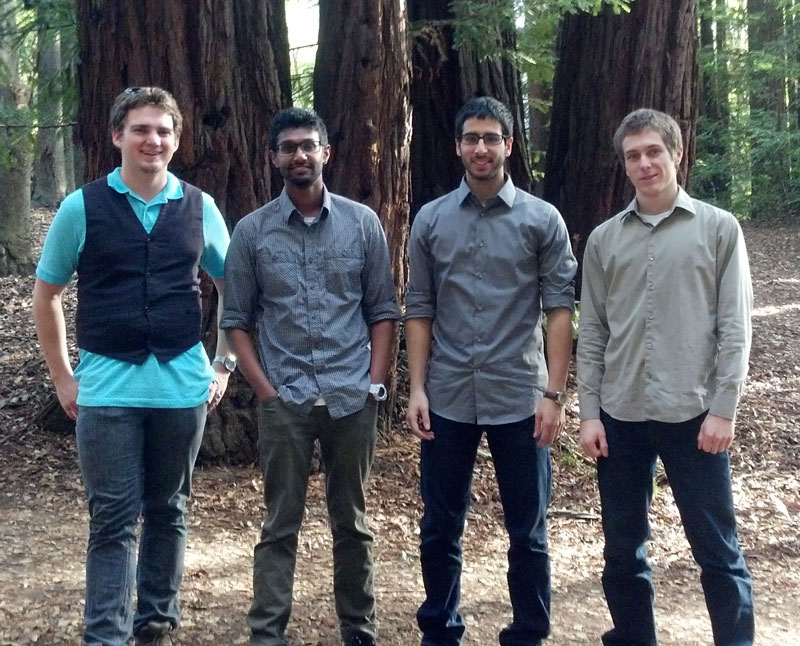
\includegraphics[width=0.42\textwidth]{group-bad1.jpg}}%
		}%
		\\	% this spacer is needed to make the text on the right fit OK
	\end{wrapfigure}
	
	\NewsItem{Who Are We}
	\emph{We are a group of UC Santa Cruz computer and robotics engineering students who are building a robot to assist lifeguards in saving drowning individuals on beaches, at sea, and in other bodies of water. In the United States, there have been a reported 99 people that have drowned in the past year alone, with a good number of them occurring while a lifeguard was on duty. We propose an autonomous boat that can navigate to a person, allowing them to hang on and stay a float until the lifeguard arrives. Our aim is to keep beaches safer by reducing the risk of drowning.}
\end{minipage}
\end{center}
% -----


% Other news (1)
% -----
\vspace{0.5cm}
	\SepRule
\vspace{0.5cm}
\begin{multicols}{3}
	\NewsItem{Progress}
	\NewsAuthor{D. Goodman}
	January has been a very productive month for our team. We are making tremendous progress on the project. Throughout January we have been hard at work writing, researching, coding, and soldering. In terms of administrative tasks, we have completed a Gantt chart, a website, and have entered into the Texas Instruments Analog Design Contest. In the hardware and software aspects, we have been progressing by leaps and bounds. Not only have we purchased a boat and begun to modify it, but we have also bought our motors, ESCs, and batteries to power the boat.  The command center---an encoded tripod assembly that the lifeguard will use to designate a drowning person---is also coming together as well. We have acquired a tripod and some absolute rotary encoders. The encoder housing has been created, and a software interface is now on-line to take angular measurements. Great care has be taken to ensure that the encoders are very precise so that we can triangulate the position of a drowning person accurately with minimal error. Many of our other sensors are nearly complete as well. We have our accelerometer up and running, our thermal sensor array nearly complete, our altimeter is working, our GPS modules are running and we are analyzing their data in MATLAB, and we have been planning our approach to implementing the microwave radar and sonar sensors after inspecting their analog waveforms with an oscilloscope. 
% -----

\vspace{1cm}
% Other news (2)
% -----
\NewsItem{Direction}
\NewsAuthor{J. Doe}
	\blindtext[1]
		\begin{center}
			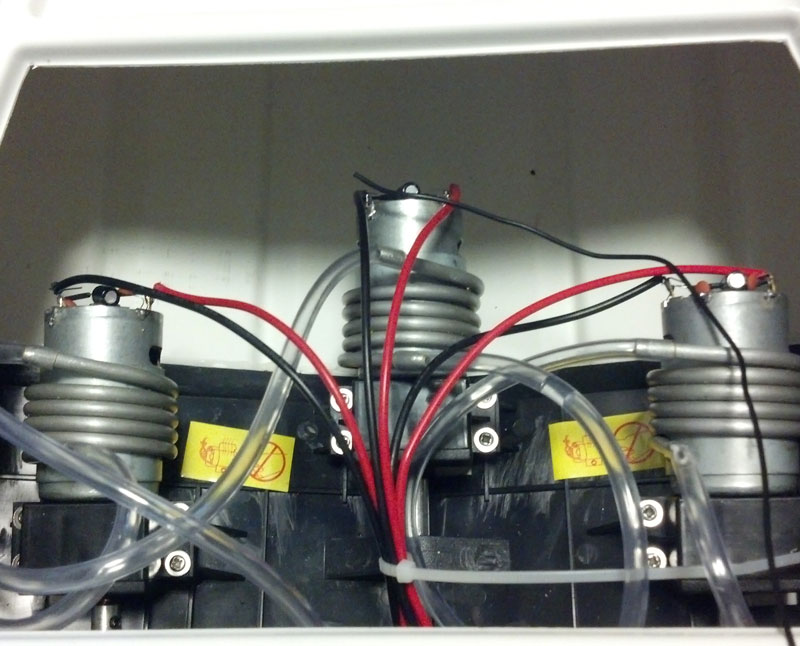
\includegraphics[width=0.78\linewidth]{old_motors.jpg}
		\end{center}
		\blindtext[1]
\end{multicols}
% -----
\end{document} 

